\documentclass[12pt]{article}
\usepackage{graphicx}
%\documentclass[journal,12pt,twocolumn]{IEEEtran}
\usepackage[none]{hyphenat}
\usepackage{graphicx}
\usepackage{listings}
\usepackage[english]{babel}
\usepackage{graphicx}
\usepackage{caption}
\usepackage[parfill]{parskip}
\usepackage{hyperref}
\usepackage{gensymb}
\usepackage{amssymb}
\usepackage[cmex10]{amsmath}
\usepackage{amsthm}
\usepackage{booktabs}
%\usepackage{setspace}\doublespacing\pagestyle{plain}
\def\inputGnumericTable{}
\usepackage{color} 
    \usepackage{array} 
    \usepackage{longtable}    
    \usepackage{calc}     
    \usepackage{multirow}                                      
    \usepackage{hhline}                                        
    \usepackage{ifthen}
\usepackage{array}
\usepackage{amsmath}   % for having text in math mode
\usepackage{parallel,enumitem}
\usepackage{listings}
\lstset{
language=tex,
frame=single,
breaklines=true
}
 
%Following 2 lines were added to remove the blank page at the beginning
\usepackage{atbegshi}% http://ctan.org/pkg/atbegshi
\AtBeginDocument{\AtBeginShipoutNext{\AtBeginShipoutDiscard}}
%
%New macro definitions
\providecommand{\mbf}{\mathbf}
\providecommand{\pr}[1]{\ensuremath{\Pr\left(#1\right)}}
\providecommand{\qfunc}[1]{\ensuremath{Q\left(#1\right)}}
\providecommand{\sbrak}[1]{\ensuremath{{}\left[#1\right]}}
\providecommand{\lsbrak}[1]{\ensuremath{{}\left[#1\right.}}
\providecommand{\rsbrak}[1]{\ensuremath{{}\left.#1\right]}}
\providecommand{\brak}[1]{\ensuremath{\left(#1\right)}}
\providecommand{\lbrak}[1]{\ensuremath{\left(#1\right.}}
\providecommand{\rbrak}[1]{\ensuremath{\left.#1\right)}}
\providecommand{\cbrak}[1]{\ensuremath{\left\{#1\right\}}}
\providecommand{\lcbrak}[1]{\ensuremath{\left\{#1\right.}}
\providecommand{\rcbrak}[1]{\ensuremath{\left.#1\right\}}}
\newcommand{\mydet}[1]{\ensuremath{\begin{vmatrix}#1\end{vmatrix}}}
\providecommand{\brak}[1]{\ensuremath{\left(#1\right)}}
\providecommand{\norm}[1]{\left\lVert#1\right\rVert}
\newcommand{\solution}{\noindent \textbf{Solution: }}
\newcommand{\myvec}[1]{\ensuremath{\begin{pmatrix}#1\end{pmatrix}}}
\providecommand{\abs}[1]{\left\vert#1\right\vert}
\let\vec\mathbf
\begin{document}
\begin{center}
\enlargethispage{-4cm}
\title{\textbf{Circles}}
\date{\vspace{-5ex}} %Not to print date automatically
\maketitle
\end{center}
\setcounter{page}{1}
\section*{10$^{th}$ Maths - Chapter 10}
This is Problem-3 from Exercise 1
\begin{enumerate}
\item A tangent $\vec{PQ}$ at a point $\vec{P}$ of a circle of radius 5 cm meets a line through the centre $\vec{O}$ at a point $\vec{Q}$ so that $\vec{OQ}$ = 12 cm. Length $\vec{PQ}$ is

\solution \\The input parameters for this problem are available in Table %\eqref{Table-1}
\begin{table}[ht!]\centering


\caption{}
\label{Table-1} 
\end{table}
The circle of radius 5cm and point $\vec{Q}$ at a distance 12cm from the centre. Tangent can be drawn from point $\vec{Q}$ on to the circle with point of contact $\vec{P}$.
The points of intersection of the line is given by
\begin{align}
	L: \quad \vec{x} = \vec{q} + \mu \vec{m} \quad \mu \in \mathbb{R}\label{eq:1}
\end{align}
with the conic section
\begin{align}
	\vec{x}^{\top}\vec{V}\vec{x}+2\vec{u}^{\top}\vec{x}+f=0\label{eq:2}
\end{align}
is given by
\begin{align}
	\vec{x}_i = \vec{q} + \mu_i \vec{m}\label{eq:3}
\end{align}
where
\begin{multline}
\mu_i = \frac{1}{\vec{m}^{\top}\vec{V}\vec{m}}
	\lbrak{-\vec{m}^{\top}\brak{\vec{V}\vec{q}+\vec{u}}}\\ \pm {\small \rbrak{\sqrt{\sbrak{\vec{m}^{\top}\brak{\vec{V}\vec{q}+\vec{u}}}^2-\brak{\vec{q}^{\top}\vec{V}\vec{q} + 2\vec{u}^{\top}\vec{q} +f}\brak{\vec{m}^{\top}\vec{V}\vec{m}}}}}\label{eq:4}
\end{multline}
If $L$ in \eqref{eq:1} touches \eqref{eq:2} at exactly one point $\vec{q}$, 
\begin{align}
  \vec{m}^{\top}\brak{\vec{V}\vec{q}+\vec{u}} = 0
\end{align}
		In this case, conic intersection has exactly one root.  Hence, in \eqref{eq:4}
  \begin{align}
  \sbrak{
  \vec{m}^{\top}\brak{\vec{V}\vec{q}+\vec{u}}
  }^2 -\brak{\vec{m}^{\top}\vec{V}\vec{m}}
  \brak
  {
\vec{q}^{\top}\vec{V}\vec{q} + 2\vec{u}^{\top}\vec{q} +f
	  } = 0\label{eq:6}
  \end{align}    
		So, the equation of conic can be written in the form of \eqref{eq:4} as,
\begin{align}
	\vec{x}^{\top}\myvec{1&0\\0&1}\vec{x}+2\myvec{0&0}\vec{x}-25=0 \label{eq:7}
\end{align}
		Let direction vector $\vec{m}$ be,
\begin{align}
	\vec{m}=\myvec{1 \\ \lambda}\label{eq:8}
\end{align}
and let $\vec{q}$ be the point $\vec{Q}$,
\begin{align}
	\vec{q}=\myvec{12 \\ 0}\label{eq:9}
\end{align}
		Substituting \eqref{eq:7},\eqref{eq:8} and \eqref{eq:9} in \eqref{eq:6} gives,
\begin{align}
	\sbrak{\vec{m}^{\top}\brak{\vec{V}\vec{q}}}^2 - \brak{\vec{m}^{\top}\vec{V}\vec{m}}\brak{\vec{q}^{\top}\vec{V}\vec{q}+(-25)} =0
\end{align}
\begin{align}
\implies\sbrak{\myvec{1 & \lambda}\myvec{12 \\ 0}}^2 - \brak{\myvec{1 & \lambda}\myvec{1 \\ \lambda}}\brak{\myvec{12 & 0}\myvec{12 \\ 0}-25}=0
	\end{align}      
	\begin{align}
		\implies\brak{12}^2-\brak{1+\lambda^2}\brak{144-25} &= 0\\
	\implies144 - \brak{1+\lambda^2}\brak{119} &= 0 \\
	\implies\brak{1+\lambda^2}\brak{119} &= -144 \\
	\implies\lambda &= \pm \frac{5}{\sqrt{119}}
\end{align}
Then
\begin{align}
	\vec{m} &= \myvec{1 \\ \pm \frac{5}{\sqrt{119}}}\\
	&=\myvec{1\\ \pm 0.4583}
\end{align}
From \eqref{eq:4} and \eqref{eq:6}
\begin{align}
	\mu_i &= \frac{1}{\vec{m}^{\top}\vec{V}\vec{m}}\lbrak{-\vec{m}^{\top}\brak{\vec{V}\vec{q}+\vec{u}}}\\
	&= \frac{1}{\myvec{1 & 0.4583}}\vec{I}\myvec{1 \\ 0.4583}\lbrak{-\myvec{1 & 0.4583}\brak{\vec{I}\myvec{12 \\ 0}}} \\
	&= -\frac{119}{12}\\
	&=-9.916
\end{align}
Now \eqref{eq:3} becomes,
\begin{align}
	\vec{x_i} &= \myvec{12 \\ 0}+(-9.916)\myvec{1 \\ \pm \frac{5}{\sqrt{119}}}\\
\vec{x_i} &= \myvec{12 \\ 0}+\myvec{-9.916 \\ \pm 4.545}
\end{align}
Then,
\begin{align}
\vec{x_i} = \myvec{2.083\\ \pm 4.545}
\end{align}
Therefore,
\begin{align}
\vec{P_1} = \myvec{2.083 \\ 4.545} \\
\vec{P_2} = \myvec{2.083 \\ -4.545}
\end{align}
the length of tangent $\vec{P}$ and $\vec{Q}$ is given by
\begin{align}
d&=\norm{\vec{P}-\vec{Q}}\\
	d^2&=(\vec{P}-\vec{Q})(\vec{P}-\vec{Q})^{\top}\label{eq:28}
\end{align}
Then
\begin{align}
	\vec{P}-\vec{Q}&=\myvec{2.083\\4.545}-\myvec{12\\0}\\
	&=\myvec{-9.916\\4.545}\label{eq:30}
\end{align}
Then substituting \eqref{eq:30} in \eqref{eq:28} gives
\begin{align}
	d^2&=\frac{14161}{144}+\frac{2975}{144}\\
	d&=\sqrt{119}
\end{align}
\begin{figure}[!h]
 \begin{center}
 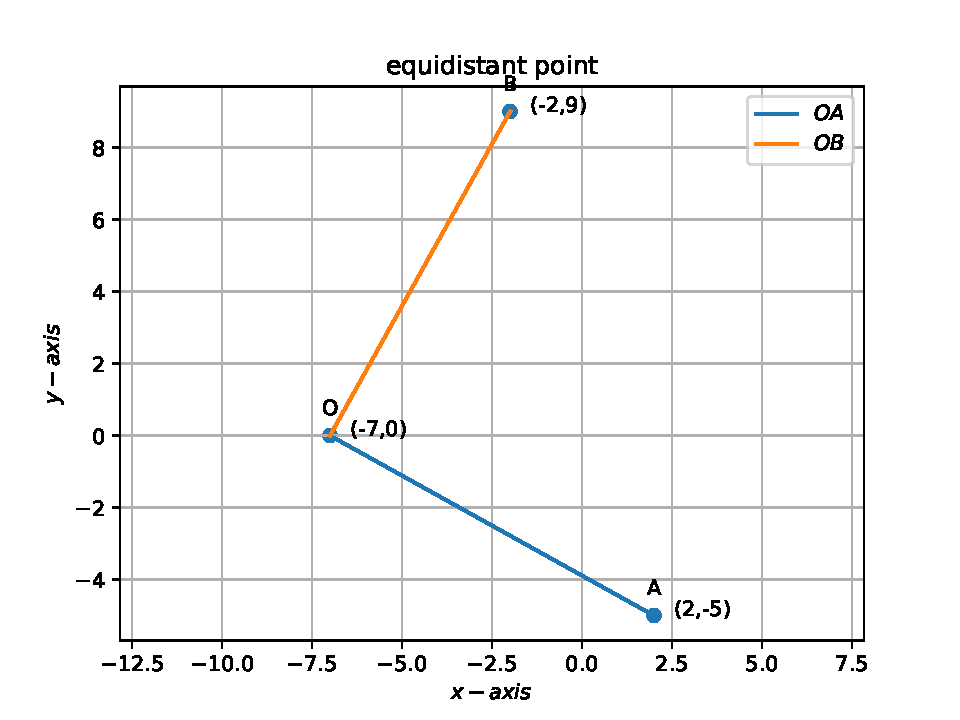
\includegraphics[width=\columnwidth]{figs/fig.pdf}
 \end{center}
\caption{}
\label{fig:Fig1}
\end{figure}
\end{enumerate}
\end{document}
